\documentclass[12pt, letterpaper]{article}

\usepackage[english]{babel} % Sets the language and regional settings for English documents
\usepackage[utf8]{inputenc} % Allows the use of UTF-8 characters in the document
\usepackage[T1]{fontenc} % Specifies t\subsubsection*{Forma canónica reducida}
\usepackage[margin=2cm]{geometry} % Sets the page margins
\usepackage{makeidx} % Enables the creation of indexes
% \usepackage{natbib} % Provides flexible bibliography support
\usepackage{url} % Allows the use of URLs
\usepackage{enumitem} % Customizes the appearance of lists
\usepackage{listings} % Provides syntax highlighting for code listings
\usepackage[dvipsnames]{xcolor} % Allows the use of colors
\usepackage{parskip} % Modifies paragraph spacing
\usepackage{graphicx} % Enables the inclusion of graphics
\usepackage{tikz} % Allows the creation of graphics and diagrams
\usepackage{float}
\usepackage{hyperref} % Enables the creation of hyperlinks
\usepackage{amsmath} % Provides additional math environments and commands
\usepackage{circuitikz} % Allows the creation of electrical circuits
\usepackage{adjustbox} % Adjusts the size of the circuit diagrams
\usepackage{tcolorbox}
\usepackage{diagbox} % Allows the use of diagonal boxes in table cells
\usepackage{colortbl} % Allows coloring of table cells
\hypersetup{
    colorlinks=true,
    linkcolor=blue,
    urlcolor=blue
}
\usepackage{breakurl} % permite que los links se rompan en varias líneas
\definecolor{mygray}{gray}{0.9}

\usetikzlibrary{shapes.geometric, positioning}

\lstset{
	language=SQL,
	basicstyle=\ttfamily\small,
	keywordstyle=\color{blue},
	commentstyle=\color[rgb]{0,0.5,0},
	stringstyle=\color{red},
	numbers=left,
	numberstyle=\tiny\color{gray},
	stepnumber=1,
	numbersep=10pt,
	backgroundcolor=\color{white},
	showspaces=false,
	showstringspaces=false,
	breaklines=true,
	frame=single,
	tabsize=2, captionpos=b, lineskip=-1pt,
	extendedchars=true,
	literate={á}{{\'a}}1 {é}{{\'e}}1 {í}{{\'i}}1 {ó}{{\'o}}1 {ú}{{\'u}}1 {Á}{{\'A}}1 {É}{{\'E}}1 {Í}{{\'I}}1 {Ó}{{\'O}}1 {Ú}{{\'U}}1 {ñ}{{\~n}}1 {Ñ}{{\~N}}1 {¿}{{\textquestiondown}}1 {¡}{{\textexclamdown}}1
}

% VHDL language configuration
\lstdefinelanguage{VHDL}{
	morekeywords={entity, architecture, signal, port, in, out, inout, begin, end, process, if, then, else, elsif, case, when, others, for, while, loop, wait, library, use, std_logic, std_logic_vector, integer, boolean, rising_edge, falling_edge, component, generic, map, downto, to, and, or, not, xor, nand, nor, xnor},
	morecomment=[l]{--},
	morestring=[b]",
	sensitive=false,
	alsoletter={_}
}

% VHDL listings style
\lstdefinestyle{vhdl}{
	language=VHDL,
	basicstyle=\ttfamily\small,
	keywordstyle=\color{blue}\bfseries,
	commentstyle=\color[rgb]{0,0.6,0}\itshape,
	stringstyle=\color{red},
	numbers=left,
	numberstyle=\tiny\color{gray},
	stepnumber=1,
	numbersep=10pt,
	backgroundcolor=\color{white},
	showspaces=false,
	showstringspaces=false,
	breaklines=true,
	frame=single,
	tabsize=2,
	captionpos=b,
	lineskip=-1pt,
	extendedchars=true
}

\graphicspath{ {./img/} } % Sets the path for the graphics

\newlist{biblio}{enumerate}{1}
\setlist[biblio,1]{label=[\arabic*]}

\makeindex

\begin{document}

\begin{titlepage}

	\begin{tikzpicture}[remember picture,overlay]
		\node[anchor=north west, inner sep=30] at (current page.north west) {
			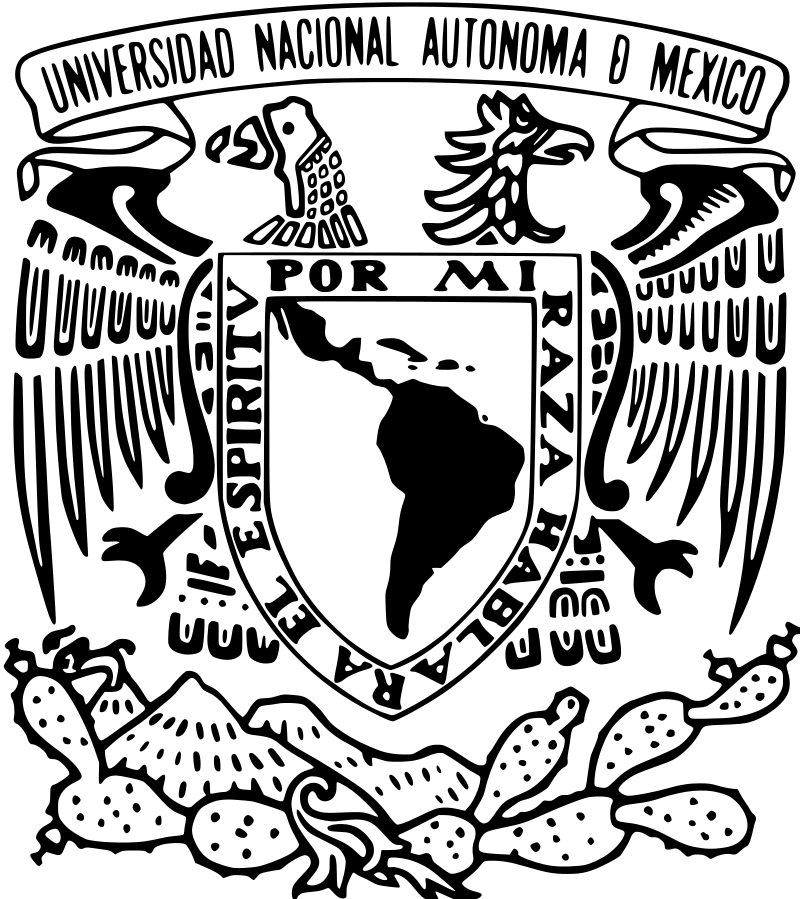
\includegraphics[width=4cm]{escudoUNAM.png}
		};

		\node[anchor=north east, inner sep=30] at (current page.north east) {
			
\includegraphics[width=4cm]{escudoFI.png}
		};
	\end{tikzpicture}

	\begin{center}
		\vspace*{3cm}

		\Huge
		\textbf{Práctica - Medición de Potencia}\\

		\vspace{2.5cm}

		\Huge
		\textbf{Facultad de Ingeniería}\\
		Laboratorio de Circuitos Eléctricos\\
		\textbf{Martha Isela Torres Hernandez} \\
		Semeste 2026-1\\

		\vspace{2.5cm}

		%grupo de la materia
		\textbf{Grupo:} \\

		\vspace{2.5cm}

		\Huge
		Tepal Briseño Hansel Yael\\
		Ugartechea Gonzáles Luiz Antonio\\
		%fecha de entrega
		\textbf{Fecha de entrega:} 28 de Octubre del 2025\\
		\vspace{2.5cm}
	\end{center}

\end{titlepage}

% \section{Marco Teórico}

% \textbf{Investigar:}

% - Que es el triángulo de Potencia
% - Cada potencia que se compone el triángulo
% - Que componentes tienen potencia activa y reactiva
% - Factor de potencia ideal

% 0.583 kW

\section{Objetivo}

Habilitar al alumno en la medición de potencia en sistemas electricos.

\section{Introducción}

La medición de potencias en sistemas trifásicos es fundamental para el análisis y la optimización del rendimiento energético. En esta práctica, se explorarán los conceptos de potencia activa, reactiva y aparente, así como el factor de potencia, así como el angulo de desfase en diferentes configuraciones de carga.

La potencia activa (P) representa la energía útil consumida por la carga, mientras que la potencia reactiva (Q) está asociada con los campos magnéticos y eléctricos en los componentes inductivos y capacitivos. La potencia aparente (S) es la combinación vectorial de P y Q, y se expresa en voltamperios (VA). El factor de potencia (FP) es una medida de la eficiencia con la que se utiliza la energía eléctrica, definido como la relación entre la potencia activa y la potencia aparente.

Mediante la realización de experimentos prácticos, se medirán estas potencias en diferentes configuraciones de carga (resistiva, inductiva y capacitiva) y se analizará el impacto del factor de potencia en el rendimiento del sistema. Los resultados obtenidos permitirán comprender mejor la importancia de una correcta gestión de la potencia en sistemas eléctricos trifásicos.

\section{Desarrollo}

\subsection{Experimento 1}

Medición  de  la  potencia  activa  de  una  carga  resistiva  equilibrada  conectada  en estrella.

Arme  el  circuito  de  la  figura  7  y  anote  los  valores de  tensión,  corriente  y  potencia en  la  Tabla  1  en  el  renglón
correspondiente,  calcule  así  mismo  P,S  y  cos\(\phi\) ,  obteniendo  el triángulo  de  potencia  y  el diagrama  fasorial  correspondiente.

Las  resistencias  empleadas  son  focos  de  300 watts,  127 volts, por  lo  que  su  resistencia  nominal  R  es:

\begin{equation}
R = \frac{V^2}{P} = \frac{127^2}{300} = 54 \Omega
\end{equation}

Estos  focos  se  conectan  en  serie para  dar  una  resistencia  por fase  de  108 \(\Omega\).

\begin{figure}[H]
	\centering
	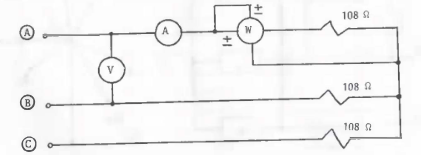
\includegraphics[width=0.6\textwidth]{Experimento1.png}
	\caption{Circuito del Experimento 1}
\end{figure}

\subsubsection{Mediciones y Resultados}

\begin{itemize}
	\item Voltaje de línea: 215.1 V
	\item Corriente: 1.562 A
	\item Resistencia por fase: 108 \(\Omega\)
	\item Potencia activa = 0.581 kW
	\item Potencia reactiva: 0.013 k VAr
	\item Potencia aparente: 0.580 k VA
	\item Factor de potencia: 1
	\item Angulo de desfase: -1.1°
\end{itemize}

\subsubsection{Triangulo de potencia}

\begin{center}
	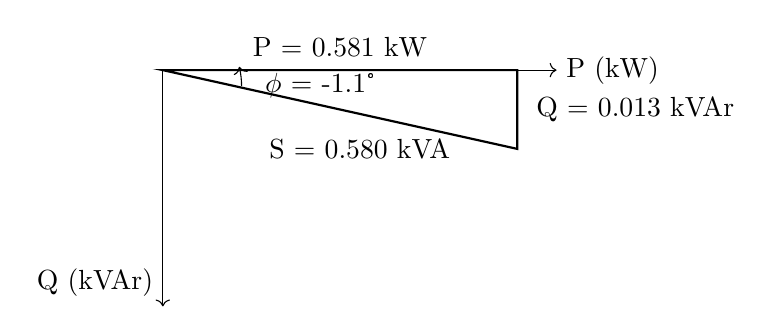
\begin{tikzpicture}[scale=1]
		% Draw axes
		\draw[->] (0,0) -- (5,0) node[right] {P (kW)};
		\draw[->] (0,0) -- (0,-3) node[above left] {Q (kVAr)};
		% Draw triangle
		\draw[thick] (0,0) -- (4.5,-0) -- (4.5,-1) -- cycle;
		% Label sides
		\node at (2.25,0.3) {P = 0.581 kW};
		\node at (6.0,-0.5) {Q = 0.013 kVAr};
		\node at (2.5,-1) {S = 0.580 kVA};
		% Angle
		\draw[->] (1,-0.2) arc[start angle=0,end angle=14,radius=1];
		\node at (2.0,-0.2) {\(\phi\) = -1.1°};

	\end{tikzpicture}
\end{center}

\subsubsection{Diagrama Fasorial}

\begin{center}
	\begin{tikzpicture}[scale=1]
		% Draw axes
		\draw[->] (0,0) -- (5,0) node[right] {V (V)};
		\draw[->] (0,0) -- (0,-3) node[above] {I (A)};
		% Draw vectors with colored lines and matching labels
		% Angle

		% Phasors: Va and Ia (reference)
		\draw[thick,->,blue]  (0,0) -- (4.5,0) node[midway, above, yshift=1pt, blue] {$V_{an}$};
		\draw[thick,->,red]   (0,0) -- ({4.5*cos(-1.1)},{4.5*sin(0)}) node[midway, below right, yshift=-1pt, red] {$I_a$};

		% Phase currents I_b and I_c (120° shifted from I_a)
		\draw[thick,->,red,dashed] (0,0) -- ({4.5*cos(-121.1)},{4.5*sin(-121.1)}) node[midway, below left, yshift=0pt, red] {$I_b$};
		\draw[thick,->,red,dashed] (0,0) -- ({4.5*cos(118.9)},{4.5*sin(118.9)}) node[midway, above left, yshift=0pt, red] {$I_c$};

		% Phase voltages V_bn and V_cn (120° shifted from V_a)
		\draw[thick,->,blue,dashed] (0,0) -- ({4.5*cos(-120)},{4.5*sin(-120)}) node[midway, below left, yshift=0pt, blue] {$V_{bn}$};
		\draw[thick,->,blue,dashed] (0,0) -- ({4.5*cos(120)},{4.5*sin(120)}) node[midway, above left, yshift=0pt, blue] {$V_{cn}$};
	\end{tikzpicture}
\end{center}

\subsection{Experimento 2}

Medición  de  la  potencia  para  la  carga  conectada  en  delta.

El  objetivo  de  este  inciso,  es  comprobar,  que  la  potencia consumida  por  una  carga  conectada  en  delta,  es  tres  vecesmayor  que  la  consumida  por  la  misma  carga  conectada  en  estrella.

Arme  el  circuito  de  la  figura  9  y  anote  los  resultados  en el  renglón  correspondiente  de  la  Tabla  1.

Obtenga  la  relación  entre  la  potencia  trifásica  de  la  conexión  en  delta  y  de  la  conexión  en  estrella.  Justifique  sus  resultados  analíticamente.

\begin{figure}[H]
	\centering
	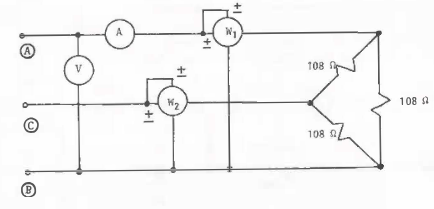
\includegraphics[width=0.6\textwidth]{Experimento2.png}
	\caption{Circuito del Experimento 2}
\end{figure}

\subsubsection{Mediciones y Resultados}

\begin{itemize}
	\item Voltaje de línea: 215.1 V
	\item Corriente: 3.730 A
	\item Resistencia por fase: 36 \(\Omega\)
	\item Potencia activa = 1.387 kW
	\item Potencia reactiva: 0.025 k VAr
	\item Potencia aparente: 1.387 k VA
	\item Factor de potencia: 1
	\item Angulo de desfase: -1.3°
\end{itemize}


\subsubsection{Comprobación de potencia entre estrella y delta}

La potencia activa medida en la conexión en estrella fue de 0.581 kW, mientras que en la conexión en delta fue de 1.387 kW.

Calculamos la relación entre ambas potencias:

\begin{equation}
\frac{P_{\Delta}}{P_Y} = \frac{1.387 kW}{0.581 kW} \approx 2.39
\end{equation}

Aunque la relación ideal debería ser 3, la diferencia puede atribuirse a pérdidas en el sistema y variaciones en las mediciones. Sin embargo, se observa que la potencia en delta es significativamente mayor que en estrella, lo cual es consistente con la teoría de conexiones trifásicas.

\subsubsection{Triangulo de potencia}

\begin{center}
	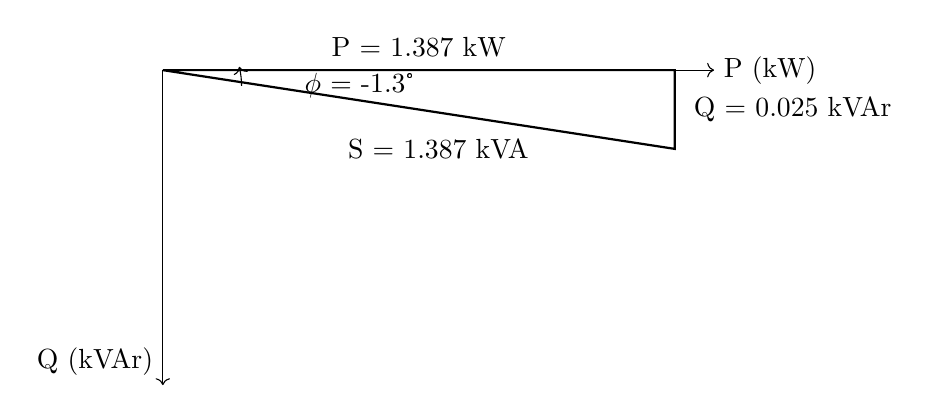
\begin{tikzpicture}[scale=1]
		% Draw axes
		\draw[->] (0,0) -- (7,0) node[right] {P (kW)};
		\draw[->] (0,0) -- (0,-4) node[above left] {Q (kVAr)};
		% Draw triangle
		\draw[thick] (0,0) -- (6.5,-0) -- (6.5,-1) -- cycle;
		% Label sides
		\node at (3.25,0.3) {P = 1.387 kW};
		\node at (8.0,-0.5) {Q = 0.025 kVAr};
		\node at (3.5,-1) {S = 1.387 kVA};
		% Angle
		\draw[->] (1,-0.2) arc[start angle=0,end angle=14,radius=1];
		\node at (2.5,-0.2) {\(\phi\) = -1.3°};
	\end{tikzpicture}
\end{center}

\subsubsection{Diagrama Fasorial}

\begin{center}
	\begin{tikzpicture}[scale=1]
		% Draw axes
		\draw[->] (0,0) -- (7,0) node[right] {V (V)};
		\draw[->] (0,0) -- (0,4) node[above] {I (A)};
		% Phasor lengths
		\def\rV{6.5}
		\def\rI{5.5}
		% Phase voltages: V_an (reference), V_bn, V_cn
		\draw[thick,->,blue] (0,0) -- (\rV,0) node[midway, above, yshift=1pt, blue] {$V_{an}$};
		\draw[thick,->,blue,dashed] (0,0) -- ({\rV*cos(-120)},{\rV*sin(-120)}) node[midway, below left, blue] {$V_{bn}$};
		\draw[thick,->,blue,dashed] (0,0) -- ({\rV*cos(120)},{\rV*sin(120)}) node[midway, above left, blue] {$V_{cn}$};
		% Phase currents: I_a has -30° phase shift; I_b and I_c are ±120° from I_a
		\draw[thick,->,red] (0,0) -- ({\rI*cos(-30)},{\rI*sin(-30)}) node[midway, below right, yshift=-1pt, red] {$I_a$};
		\draw[thick,->,red,dashed] (0,0) -- ({\rI*cos(-150)},{\rI*sin(-150)}) node[midway, below left, red] {$I_b$};
		\draw[thick,->,red,dashed] (0,0) -- ({\rI*cos(90)},{\rI*sin(90)}) node[midway, above left, red] {$I_c$};
		% Angle marker for phi = -30°
		\draw[->] (1,0) arc[start angle=0,end angle=-30,radius=1];
		\node at (2.0,-0.4) {$\phi = -30^\circ$};
	\end{tikzpicture}
\end{center}
\subsection{Experimento 3}

Medición  de  potencia en  un  motor  trifásico  conectado  en  delta Arme  el  diagrama mostrado  en  la  figura  10  y  mida  la  potencia activa  P,  la  corriente  I  y  la tensión  V  y  anote  sus  resulta­dos  en  el  renglón  correspondiente  de  la  Tabla  1.  Observe que en  este  caso  el  principio  de  la  bobina  de  tensión  del  wattmetro  2  se  conecta  a  la fase  e  y  el  final  a  la fase  B,  a  fin  de  evitar  que  el  wattmetro  marque  en  sentido  contrario,  debido  a  que  el  ángulo  \(\phi\) es mayor  que  60°.  Obtenga  las  potencias trifásicas  aparente  y  activa  y  dibuje  el  diagrama  fasorial  correspondiente.


\begin{figure}[H]
	\centering
	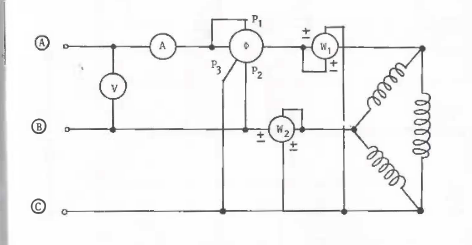
\includegraphics[width=0.6\textwidth]{Experimento3.png}
	\caption{Circuito del Experimento 3}
\end{figure}

\subsubsection{Mediciones y Resultados}

\begin{itemize}
	\item Voltaje de línea: 216.6 V
	\item Corriente: 2.282 A
	\item Potencia activa = 0.095 kW
	\item Potencia reactiva: 0.846 k VAr
	\item Potencia aparente: 0.852 k VA
	\item Factor de potencia: 0.112
	\item Angulo de desfase: 83°
\end{itemize}

\subsubsection{Triangulo de potencia}

\begin{center}
	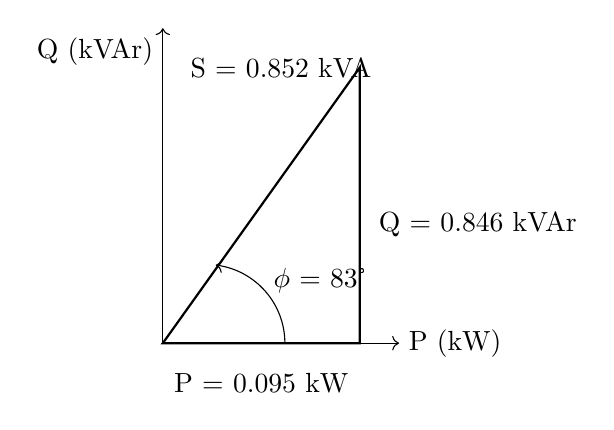
\begin{tikzpicture}[scale=1]
		% Draw axes
		\draw[->] (0,0) -- (3,0) node[right] {P (kW)};
		\draw[->] (0,0) -- (0,4) node[below left] {Q (kVAr)};
		% Draw triangle
		\draw[thick] (0,0) -- (2.5,-0) -- (2.5,3.5) -- cycle;
		% Label sides
		\node at (1.25,-0.5) {P = 0.095 kW};
		\node at (4.0,1.5) {Q = 0.846 kVAr};
		\node at (1.5,3.5) {S = 0.852 kVA};
		% Angle
		\draw[->] (1.55,0) arc[start angle=0,end angle=83,radius=1];
		\node at (2.0,0.8) {\(\phi\) = 83°};
	\end{tikzpicture}
\end{center}

\subsubsection{Diagrama Fasorial}

\begin{center}
	\begin{tikzpicture}[scale=1]
		% Draw axes
		\draw[->] (0,0) -- (7,0) node[right] {V (V)};
		\draw[->] (0,0) -- (0,6) node[above] {I (A)};
		% Phasor lengths
		\def\rV{6.5}
		\def\rI{5.5}
		% Phase voltages: V_an (reference), V_bn, V_cn
		\draw[thick,->,blue] (0,0) -- (\rV,0) node[midway, above, yshift=1pt, blue] {$V_{an}$};
		\draw[thick,->,blue,dashed] (0,0) -- ({\rV*cos(-120)},{\rV*sin(-120)}) node[midway, below left, blue] {$V_{bn}$};
		\draw[thick,->,blue,dashed] (0,0) -- ({\rV*cos(120)},{\rV*sin(120)}) node[midway, above left, blue] {$V_{cn}$};
		% Phase currents: I_a has 83° phase shift; I_b and I_c are ±120° from I_a
		\draw[thick,->,red] (0,0) -- ({\rI*cos(54.7)},{\rI*sin(54.7)}) node[midway, above right, yshift=1pt, red] {$I_a$};
		\draw[thick,->,red,dashed] (0,0) -- ({\rI*cos(-75.3)},{\rI*sin(-75.3)}) node[midway, below left, red] {$I_b$};
		\draw[thick,->,red,dashed] (0,0) -- ({\rI*cos(-185.3)},{\rI*sin(-185.3)}) node[midway, above left, red] {$I_c$};
		% Angle marker for phi = 54.7°
		\draw[->] (1,0) arc[start angle=0,end angle=54.7,radius=1];
		\node at (2.0,0.4) {$\phi = 54.7^\circ$};
	\end{tikzpicture}
\end{center}

\subsection{Experimento 4}

Medición  de  potencia  reactiva.

La  carga  es  un  banco  de  capacitares  conectados  en  paralelo para  formar  una  reactancia capacitiva  por fase  de  172.24 \(\mu F\) a  una  frecuencia  de  60Hz  y  a  su  vez,  éstas  reactancias  se conectan  en  delta  según  el esquema  de  la  figura  11.

Como  se  explicó  en  la introducción  teórica,  para  medir  potencia reactiva  es necesario  defasar  90°  la  tensión  en  la
bobina  del  wattmetro;  esto  se  consigue  en el  sistema  trifásico  conectando  la bobina  de  tensión  entre  las fases  B  y  C  en  lugar  de  hacerlo entre  las  fases  A  y  e,  como  se muestra  en  la figura 11,  ya  que  la  carga  es  equilibrada, se  utilizará  un  solo wattmetro  para  determinar  la  potencia  trifásica. B  y  C  en  lugar  de  hacerlo entre  las  fases  A  y  e,  como  se muestra  en  la figura  11,  ya  que  la  carga  es  equilibrada, se  utilizará  un  solo wattmetro  para  determinar  la  potencia trifásica.

\begin{center}
	\begin{figure}[H]
		\centering
		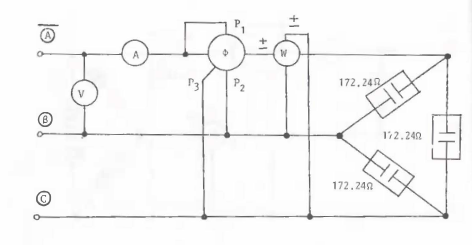
\includegraphics[width=0.6\textwidth]{Experimento4.png}
		\caption{Circuito del Experimento 4}
	\end{figure}
\end{center}

\subsubsection{Mediciones y Resultados}

\begin{itemize}
	\item Voltaje de línea: 216.2 V
	\item Corriente: 3.504 A
	\item item Potencia activa = 0.045 kW
	\item Potencia reactiva: 1.311 k VAr
	\item Potencia aparente: 1.310 k VA
	\item Factor de potencia: 0.0027
	\item Angulo de desfase: -88.1°
\end{itemize}

\subsubsection{Triangulo de potencia}
\begin{center}
	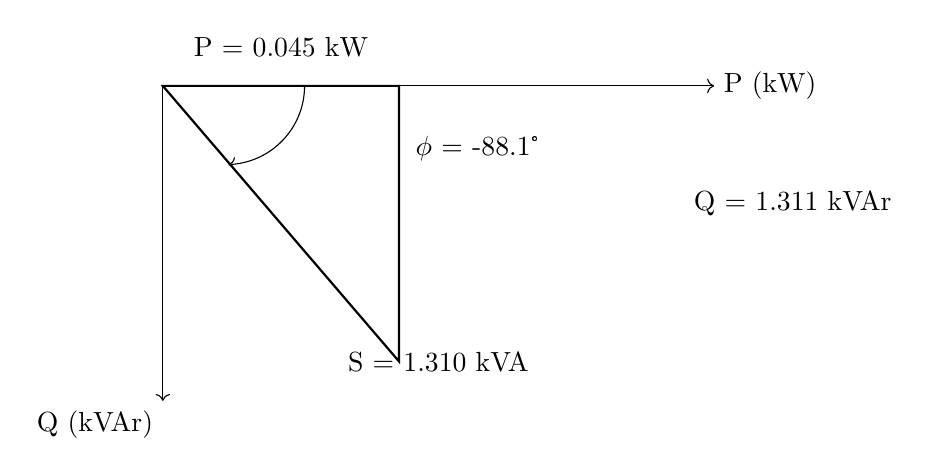
\begin{tikzpicture}[scale=1]
		% Draw axes
		\draw[->] (0,0) -- (7,0) node[right] {P (kW)};
		\draw[->] (0,0) -- (0,-4) node[below left] {Q (kVAr)};
		% Draw triangle
		\draw[thick] (0,0) -- (3,-0) -- (3,-3.5) -- cycle;
		% Label sides
		\node at (1.5,0.5) {P = 0.045 kW};
		\node at (8.0,-1.5) {Q = 1.311 kVAr};
		\node at (3.5,-3.5) {S = 1.310 kVA};
		% Angle
		\draw[->] (1.8,0) arc[start angle=0,end angle=-88.1,radius=1];
		\node at (4,-0.8) {\(\phi\) = -88.1°};
	\end{tikzpicture}
\end{center}

\subsubsection{Diagrama Fasorial}
\begin{center}
	\begin{tikzpicture}[scale=1]
		% Draw axes
		\draw[->] (0,0) -- (7,0) node[right] {V (V)};
		\draw[->] (0,0) -- (0,6) node[above] {I (A)};
		% Phasor lengths
		\def\rV{6.5}
		\def\rI{5.5}
		% Phase voltages: V_an (reference), V_bn, V_cn
		\draw[thick,->,blue] (0,0) -- (\rV,0) node[midway, above, yshift=1pt, blue] {$V_{an}$};
		\draw[thick,->,blue,dashed] (0,0) -- ({\rV*cos(-120)},{\rV*sin(-120)}) node[midway, below left, blue] {$V_{bn}$};
		\draw[thick,->,blue,dashed] (0,0) -- ({\rV*cos(120)},{\rV*sin(120)}) node[midway, above left, blue] {$V_{cn}$};
		% Phase currents: I_a has -88.1° phase shift; I_b and I_c are ±120° from I_a
		\draw[thick,->,red] (0,0) -- ({\rI*cos(-57.8)},{\rI*sin(-57.8)}) node[midway, below right, yshift=-1pt, red] {$I_a$};
		\draw[thick,->,red,dashed] (0,0) -- ({\rI*cos(62.2)},{\rI*sin(62.2)}) node[midway, above left, red] {$I_b$};
		\draw[thick,->,red,dashed] (0,0) -- ({\rI*cos(182.2)},{\rI*sin(182.2)}) node[midway, above left, red] {$I_c$};
		% Angle marker for phi = -88.1°
		\draw[->] (1,0) arc[start angle=0,end angle=-88.1,radius=1];
		\node at (2.0,-0.4) {$\phi = -88.1^\circ$};
	\end{tikzpicture}
\end{center}

\subsubsection{Calculo de la capacitancia}

\begin{equation}
C = \frac{1}{j \omega Z_C} = \frac{1}{j 2 \pi (60 Hz) (-j172.24 \Omega)} = 15.4 \mu F
\end{equation}

\subsubsection{Tabla de datos medidos}

\begin{table}[H]
	\centering
	\small % reduce font so the table fits better
	\begin{adjustbox}{max width=\textwidth}
		\begin{tabular}{|l|c|c|c|c|c|c|c|}
			\hline
			\textbf{Conexión} & \textbf{V (V)} & \textbf{I (A)} & \textbf{P (kW)} & \textbf{Q (kVAr)} & \textbf{S (kVA)} & \textbf{FP} & \(\boldsymbol{\phi}\) (°) \\
			\hline
			Carga resistiva balanceada estrella & 215.1 & 1.562 & 0.581 & 0.013 & 0.580 & 1 & -1.1 \\
			\hline
			Carga resistiva balanceada delta & 215.1 & 3.730 & 1.387 & 0.025 & 1.387 & 1 & -1.0 \\
			\hline
			Motor de inducción conectado delta & 216.6 & 2.282 & 0.095 & 0.846 & 0.852 & 0.112 & 83 \\
			\hline
			Carga capacitiva conectada delta & 216.2 & 3.504 & 0.045 & 1.311 & 1.310 & 0.0027 & -88.1 \\
			\hline
		\end{tabular}
	\end{adjustbox}
	\caption{Datos medidos en los experimentos}
\end{table}

\section{Conclusiones}

\subsection{Tepal Briseño Hansel Yael}

En esta práctica, hemos aprendido a medir y analizar las potencias en sistemas trifásicos, comprendiendo la importancia de la potencia activa, reactiva y aparente. La experiencia práctica nos ha permitido visualizar cómo diferentes configuraciones de carga afectan el rendimiento del sistema eléctrico. Además, hemos visto cómo el factor de potencia influye en la eficiencia energética, lo que es crucial para optimizar el consumo eléctrico en aplicaciones industriales y comerciales. Esta práctica ha reforzado nuestros conocimientos teóricos y nos ha proporcionado habilidades prácticas esenciales para futuros trabajos en el campo de la ingeniería eléctrica.

\subsection{Ugartechea Gonzáles Luis Antonio}

La práctica de medición de potencia en sistemas trifásicos ha sido una experiencia enriquecedora que nos ha permitido aplicar conceptos teóricos en un entorno práctico. A través de los diferentes experimentos, hemos podido observar cómo las cargas resistivas, inductivas y capacitivas afectan las mediciones de potencia y el factor de potencia. La comprensión del triángulo de potencia y la representación fasorial nos ha ayudado a visualizar las relaciones entre las diferentes formas de potencia. Esta experiencia es fundamental para nuestro desarrollo como ingenieros eléctricos, ya que nos prepara para enfrentar desafíos reales en el diseño y análisis de sistemas eléctricos eficientes.

% \section{Bibliografía}
% \renewcommand{\refname}{}
% \begin{thebibliography}{9}
%    \bibitem{} Dr. E. García, \textit{"Diseño Digital VLSI Repaso DDM"}, presentado en el curso de Diseño Digital VLSI, Ciudad de México, 2025.
% \end{thebibliography}

\end{document}
